\documentclass[tikz, border=12pt]{standalone}
\usepackage[utf8]{inputenc}
\usepackage[T5]{fontenc}
\usepackage{lmodern}
\usepackage{xcolor}
\usepackage{graphicx}
\usetikzlibrary{positioning, calc, arrows}

\definecolor{boxBorder}{RGB}{180, 195, 215}
\definecolor{tier1Bg}{RGB}{242, 250, 245}
\definecolor{tier2Bg}{RGB}{242, 247, 255}
\definecolor{tier3Bg}{RGB}{248, 245, 255}

\definecolor{greenTitle}{RGB}{27, 94, 32}
\definecolor{blueTitle}{RGB}{30, 58, 138}
\definecolor{purpleTitle}{RGB}{95, 30, 180}
\definecolor{arrowColor}{RGB}{50, 65, 85}

\begin{document}
\begin{tikzpicture}[
  >=stealth,
  font=\sffamily,
  tierContainer/.style={
    draw=boxBorder,
    line width=1.0pt,
    rounded corners=8pt,
    inner sep=10pt,
    align=center
  },
  itemCard/.style={
    draw=gray!30,
    line width=0.6pt,
    fill=white,
    rounded corners=5pt,
    align=center,
    inner sep=5pt
  },
  flowArrow/.style={
    ->,
    line width=1.4pt,
    draw=arrowColor
  },
  biArrow/.style={
    <->,
    line width=1.4pt,
    draw=arrowColor
  },
  tagLbl/.style={
    font=\small\bfseries,
    fill=white,
    inner sep=3.0pt,
    rounded corners=3pt,
    draw=gray!35,
    line width=0.5pt,
    text=arrowColor
  }
]

% ----------------- TẦNG 1: NẸP ĐEO & CƠ CẤU TRỢ LỰC -----------------
\node[tierContainer, fill=tier1Bg, text width=15.2cm] (t1) at (0, 0) {
  {\bfseries\large\color{greenTitle} NHÓM 1: TẦNG NẸP ĐEO \& CƠ CẤU TRỢ LỰC}\\[8pt]
  \begin{tikzpicture}
    % Sub-item 1: Khung nẹp 3D
    \node[itemCard, text width=4.3cm] (c1) at (-4.8, 0) {
      {\bfseries\small Khung nẹp 3D ngàm xoay}\\[2pt]
      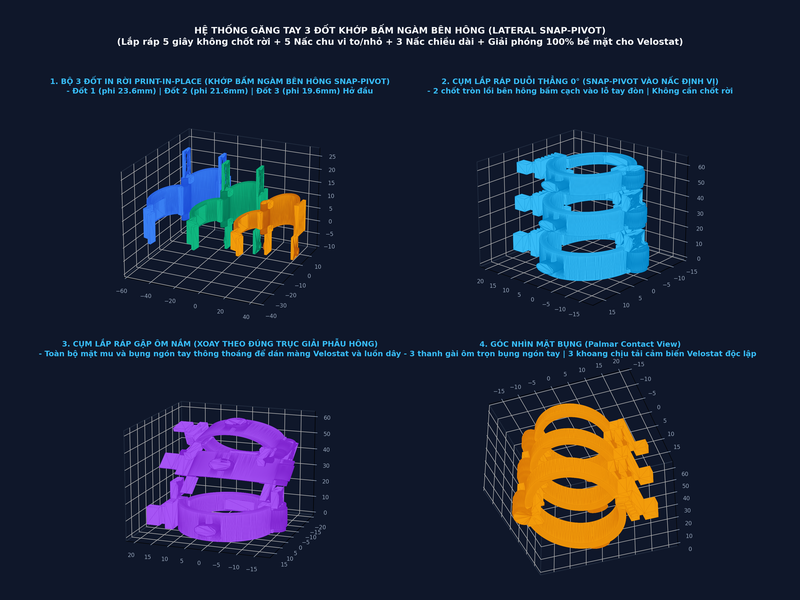
\includegraphics[width=3.9cm, height=2.2cm, keepaspectratio]{assets/splint_3d.png}\\[2pt]
      {\scriptsize Khớp bản lề kép \& Chốt mở nhanh}
    };
    % Sub-item 2: Khóa ngàm đốt nẹp
    \node[itemCard, text width=4.3cm] (c2) at (0, 0) {
      {\bfseries\small Cụm cảm biến vi sai}\\[2pt]
      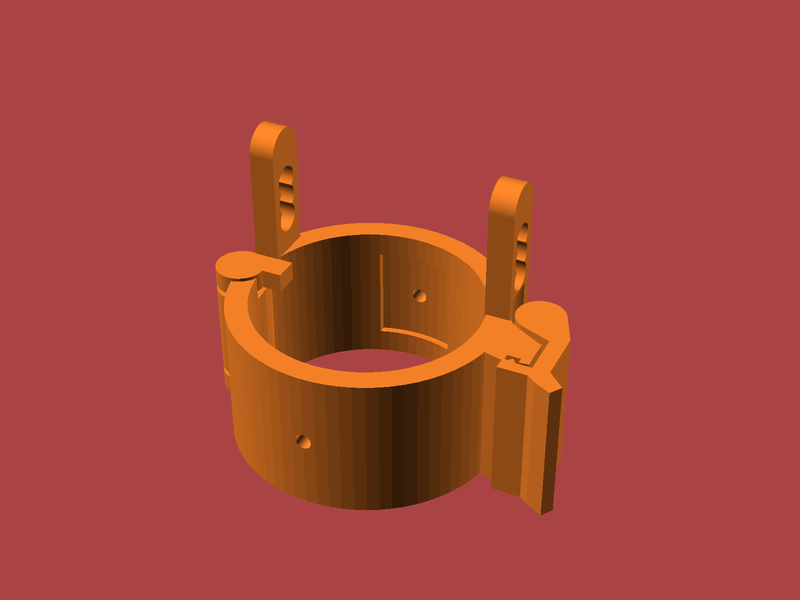
\includegraphics[width=3.9cm, height=2.2cm, keepaspectratio]{assets/mech9.png}\\[2pt]
      {\scriptsize 16 Ô Velostat + 3 Flex uốn ngón}
    };
    % Sub-item 3: Cơ cấu 3 tang servo
    \node[itemCard, text width=4.3cm] (c3) at (4.8, 0) {
      {\bfseries\small Cụm 3 Tang cuốn cáp}\\[2pt]
      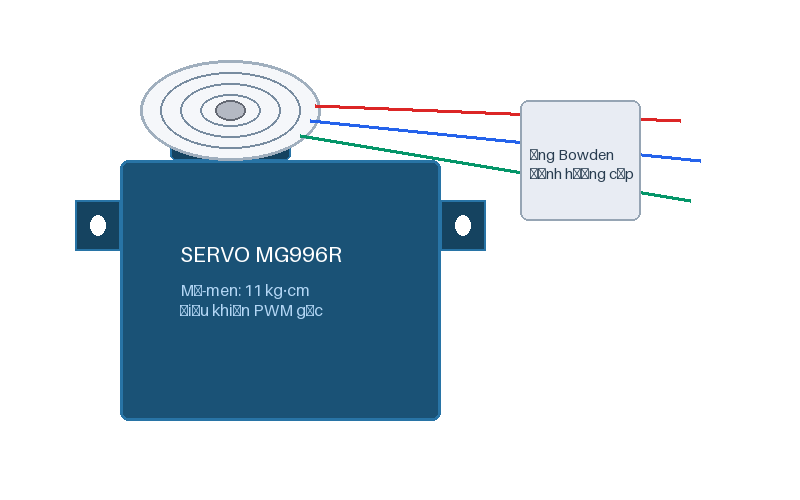
\includegraphics[width=3.9cm, height=2.2cm, keepaspectratio]{assets/servo_spool_assembly.png}\\[2pt]
      {\scriptsize Dây kéo Bowden \& Nẹp hồi vị mu}
    };
  \end{tikzpicture}
};

% ----------------- TẦNG 2: THU THẬP ĐA KÊNH & XỬ LÝ DSP -----------------
\node[tierContainer, fill=tier2Bg, text width=15.2cm, below=28pt of t1] (t2) {
  {\bfseries\large\color{blueTitle} NHÓM 2: TẦNG THU THẬP ĐA KÊNH \& XỬ LÝ SỐ DSP}\\[8pt]
  \begin{tikzpicture}
    \node[itemCard, text width=13.8cm] (c_dsp) at (0, 0) {
      {\bfseries\small Mạch tích hợp ESP32-S3 + 2 CD74HC4067 + ADC ADS1115 (16-bit, I2C trực tiếp)}\\[3pt]
      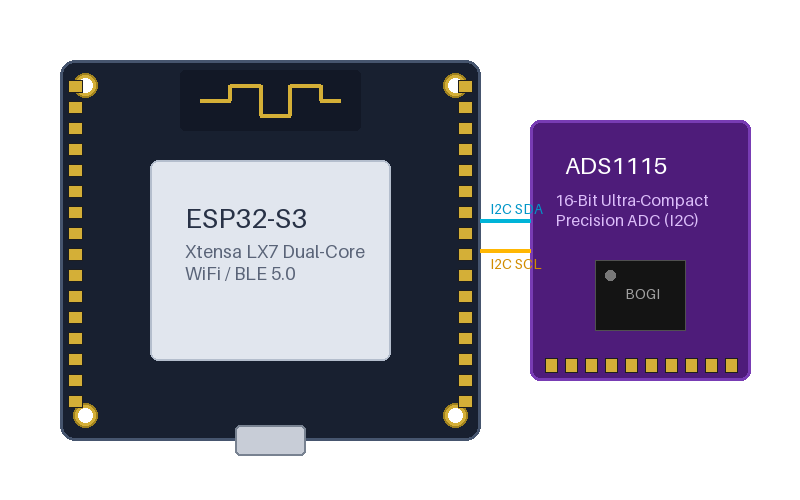
\includegraphics[width=8.5cm, height=2.6cm, keepaspectratio]{assets/controller_ads_board.png}\\[3pt]
      {\scriptsize Quét 21 kênh $\ge$15 Hz $\bullet$ Lọc số DSP 2 nhánh $\bullet$ Tính toán nỗ lực EI -- GAP -- RAL \& Thuật toán AAN}
    };
  \end{tikzpicture}
};

% ----------------- TẦNG 3: THỊ GIÁC KHÔNG GIAN 3D -----------------
\node[tierContainer, fill=tier3Bg, text width=15.2cm, below=28pt of t2] (t3) {
  {\bfseries\large\color{purpleTitle} NHÓM 3: TẦNG THỊ GIÁC KHÔNG GIAN 3D \& LƯỢNG HÓA TÁC VỤ}\\[8pt]
  \begin{tikzpicture}
    \node[itemCard, text width=13.8cm] (c_vis) at (0, 0) {
      {\bfseries\small Máy tính nhúng Orange Pi 5 Pro (NPU) + Camera RGB + Depth Anything V2}\\[3pt]
      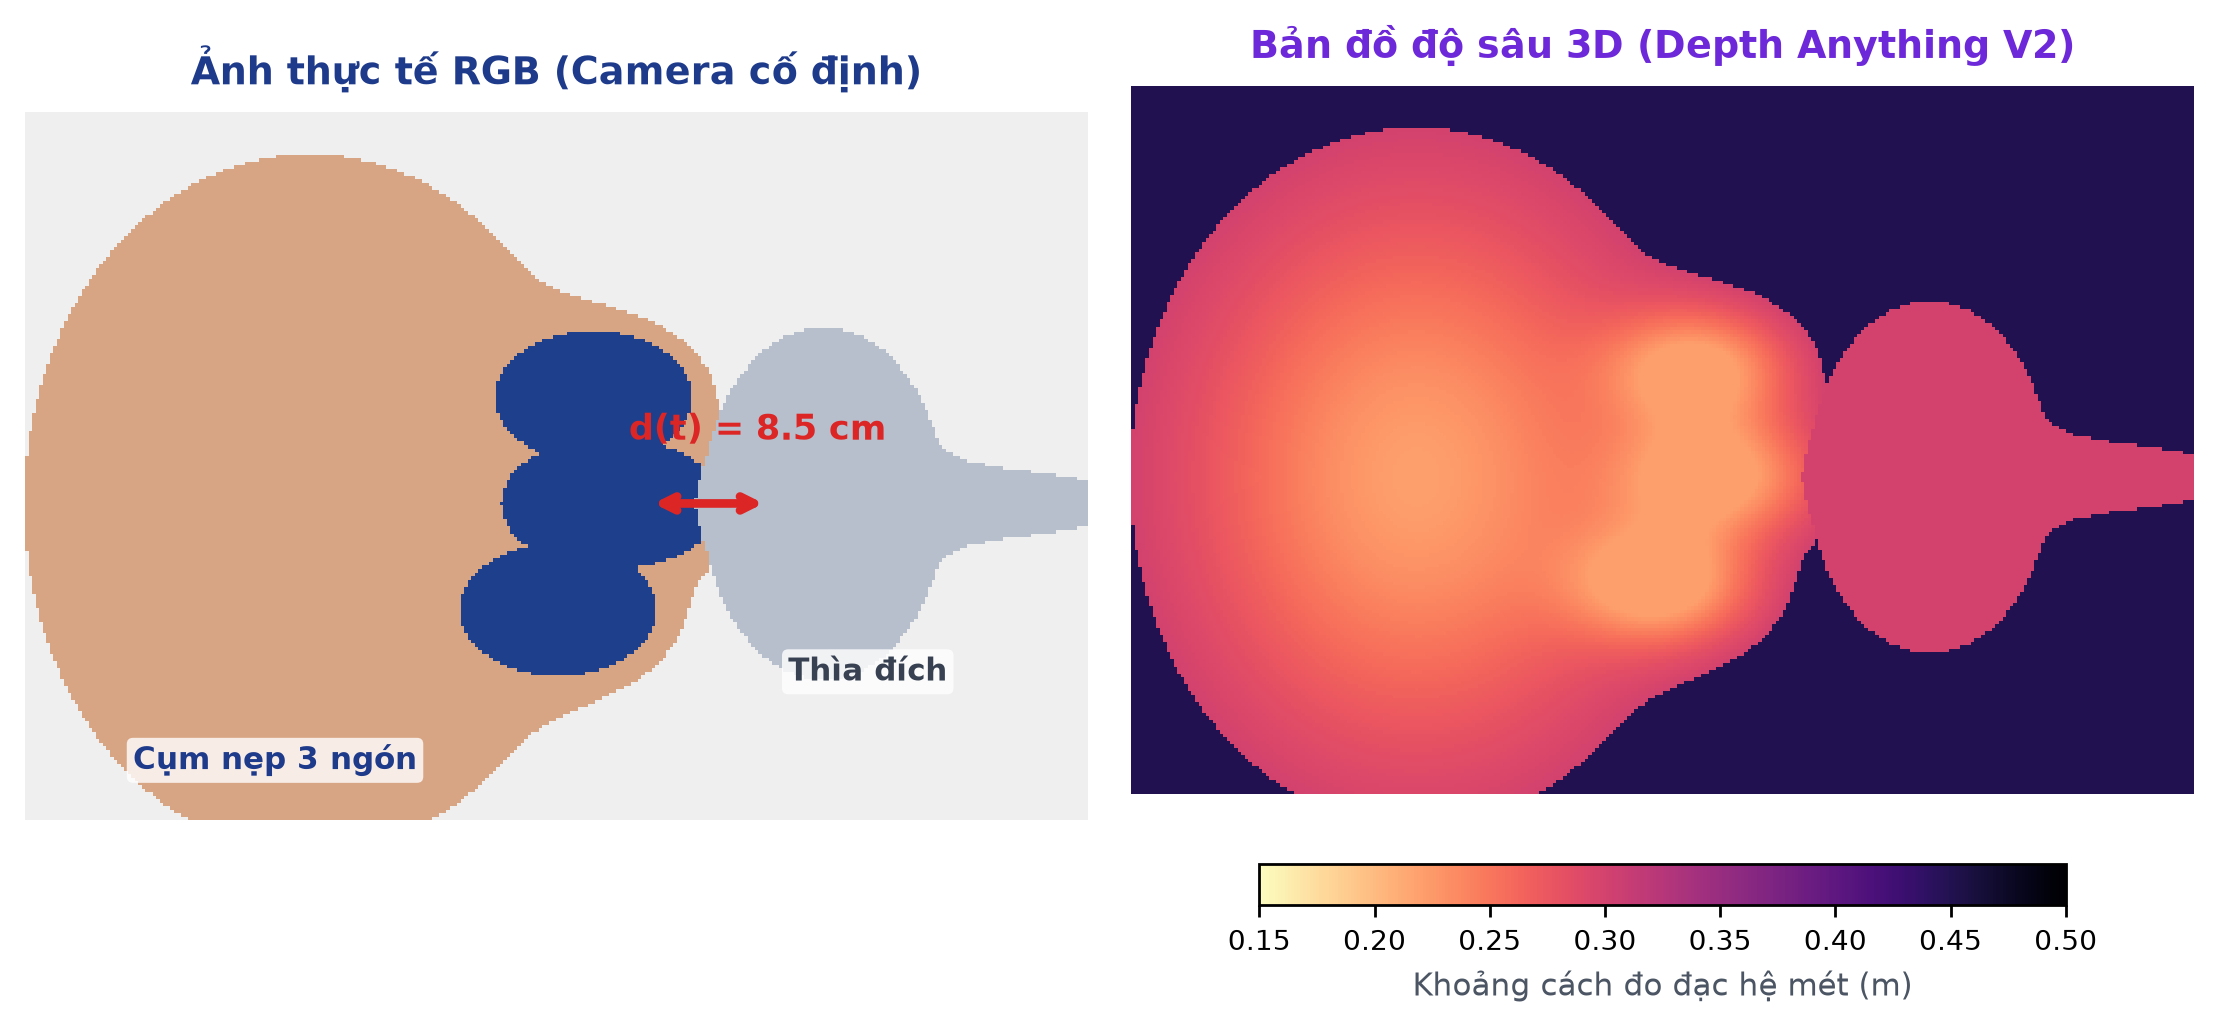
\includegraphics[width=9.5cm, height=2.8cm, keepaspectratio]{assets/depth_anything_scene.png}\\[3pt]
      {\scriptsize Ước lượng cự ly 3D tay -- vật $d(t)$ $\bullet$ Dự báo thời gian tới tiếp xúc TTC đón trước $\bullet$ Đánh giá bài tập kẹp thìa}
    };
  \end{tikzpicture}
};

% MŨI TÊN LIÊN KẾT GIỮA CÁC TẦNG
\draw[flowArrow] (t1.south) -- node[tagLbl] {Tín hiệu tương tự 21 kênh (Áp lực vi sai \& Góc gập)} (t2.north);
\draw[biArrow] (t2.south) -- node[tagLbl] {Lệnh trợ lực đón trước AAN $\longleftrightarrow$ Cự ly 3D \& Định thời TTC} (t3.north);

\end{tikzpicture}
\end{document}
